\documentclass[15pt,a5paper,reqno]{article}
\usepackage{hyperref}
\usepackage[warn]{mathtext}
\usepackage[utf8x]{inputenc}
\usepackage{amssymb, amsmath, multicol}
\usepackage[russian]{babel}
\usepackage{graphicx}
\usepackage[shortcuts,cyremdash]{extdash}
\usepackage{wrapfig}
\usepackage{floatflt}
\usepackage{lipsum}
\usepackage{verbatim}
\usepackage{concmath}
\usepackage{euler}
\usepackage{xcolor}
\usepackage{etoolbox}
\usepackage{fancyhdr}
\usepackage{subfiles}
\usepackage{enumitem}
\usepackage{amsthm}
\usepackage{indentfirst}
\usepackage{import}

\DeclareMathOperator{\sign}{sign}

\RequirePackage[ left     = 1.5cm,
  right    = 1.5cm,
  top      = 2.0cm,
  bottom   = 1.25cm,
  includefoot,
  footskip = 1.25cm ]{geometry}
\setlength    {\parskip}        { .5em plus .15em minus .08em }
%\setlength    {\parindent}      { .0em }
\renewcommand {\baselinestretch}{ 1.07 }

\fancyhf{}

\renewcommand{\footrulewidth}{ .0em }
\fancyfoot[C]{\texttt{\textemdash~\thepage~\textemdash}}
\fancyhead[R]{\hfilШурыгин}

\makeatletter
\patchcmd\l@section{%
  \nobreak\hfil\nobreak
}{%
  \nobreak
  \leaders\hbox{%
    $\m@th \mkern \@dotsep mu\hbox{.}\mkern \@dotsep mu$%
  }%
  \hfill
  \nobreak
}{}{\errmessage{\noexpand\l@section could not be patched}}
\makeatother
\parindent = 1cm % отступ при красной строке⏎
\pagestyle{fancy}    
\renewcommand\qedsymbol{$\blacksquare$}

\newcommand{\when}[2]{
  \left. #1 \right|_{#2} \hspace
}
\renewcommand{\kappa}{\varkappa}
\RequirePackage{caption2}
\renewcommand\captionlabeldelim{}
\newcommand*{\hm}[1]{#1\nobreak\discretionary{}

\DeclareSymbolFont{T2Aletters}{T2A}{cmr}{m}{it}
{\hbox{$\mathsurround=0pt #1$}}{}}
% Цвета для гиперссылок
\definecolor{linkcolor}{HTML}{000000} % цвет ссылок
\definecolor{urlcolor}{HTML}{799B03} % цвет гиперссылок
 
\hypersetup{pdfstartview=FitH,  linkcolor=linkcolor,urlcolor=urlcolor, colorlinks=true}


%\setcounter{secnum[utf8x]depth}{0}

\begin{document}

% НАЧАЛО ТИТУЛЬНОГО ЛИСТА
\begin{center}
  {\small ФЕДЕРАЛЬНОЕ ГОСУДАРСТВЕННОЕ АВТОНОМНОЕ ОБРАЗОВАТЕЛЬНОЕ\\ УЧРЕЖДЕНИЕ ВЫСШЕГО ОБРАЗОВАНИЯ\\ МОСКОВСКИЙ ФИЗИКО-ТЕХНИЧЕСКИЙ ИНСТИТУТ\\ (НАЦИОНАЛЬНЫЙ ИССЛЕДОВАТЕЛЬСКИЙ УНИВЕРСИТЕТ)\\ ФИЗТЕХ-ШКОЛА РАДИОТЕХНИКИ И КИБЕРНЕТИКИ}\\
  \hfill \break
  \hfill \break
  \hfill \break
  \Huge{Лабораторная работа 19. \\ Активные фильтры.}\\
\end{center}

\hfill \break
\hfill \break
\hfill \break
\hfill \break
\hfill \break
\hfill \break

\begin{flushright}
  \normalsize{Работу выполнил:}\\
  \normalsize{\textbf{Шурыгин Антон Алексеевич, группа Б01-909}}\\
\end{flushright}

\begin{center}
  \normalsize{\textbf{Долгопрудный, 2021}}
\end{center}


\thispagestyle{empty} % выключаем отображение номера для этой страницы

% КОНЕЦ ТИТУЛЬНОГО ЛИСТА

\newpage
\thispagestyle{plain}
\tableofcontents
\thispagestyle{plain}
\newpage



\begin{figure}[h!]
    \centering
    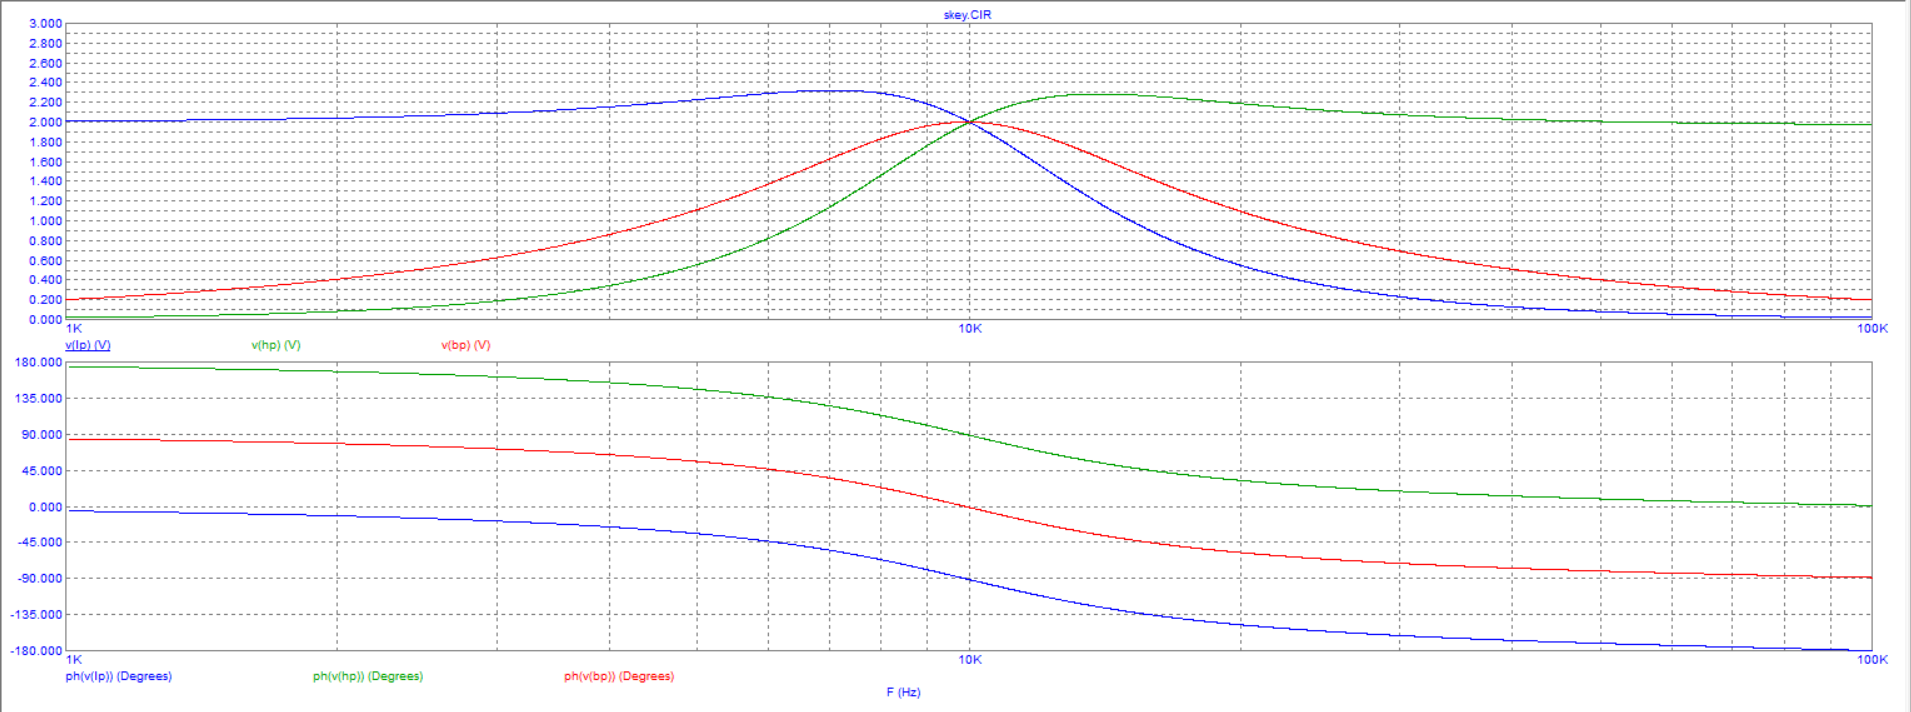
\includegraphics[width=12cm]{pics/point4.png}
    \caption{}
    \label{Задание 4 пункт 1. частотные характеристики фнч фвч и пф}
\end{figure}



\begin{figure}[h!]
    \centering
    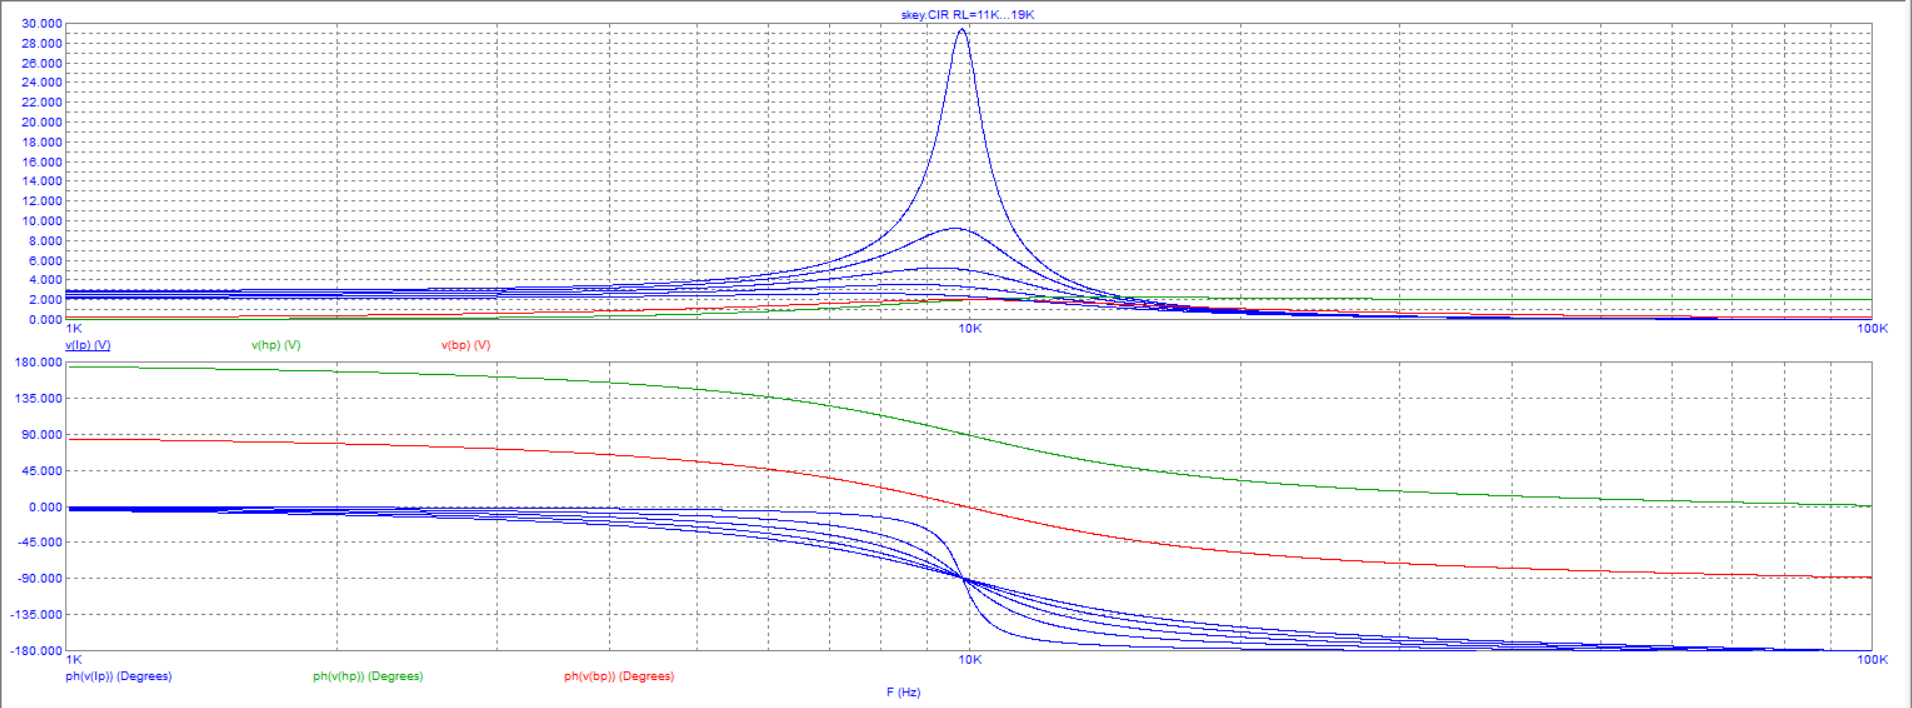
\includegraphics[width=12cm]{pics/point4_1_var1.png}
    \caption{Варьирование $R_l = [11K, 19K | 2K]$}
    \label{}
\end{figure}



\begin{figure}[h!]
    \centering
    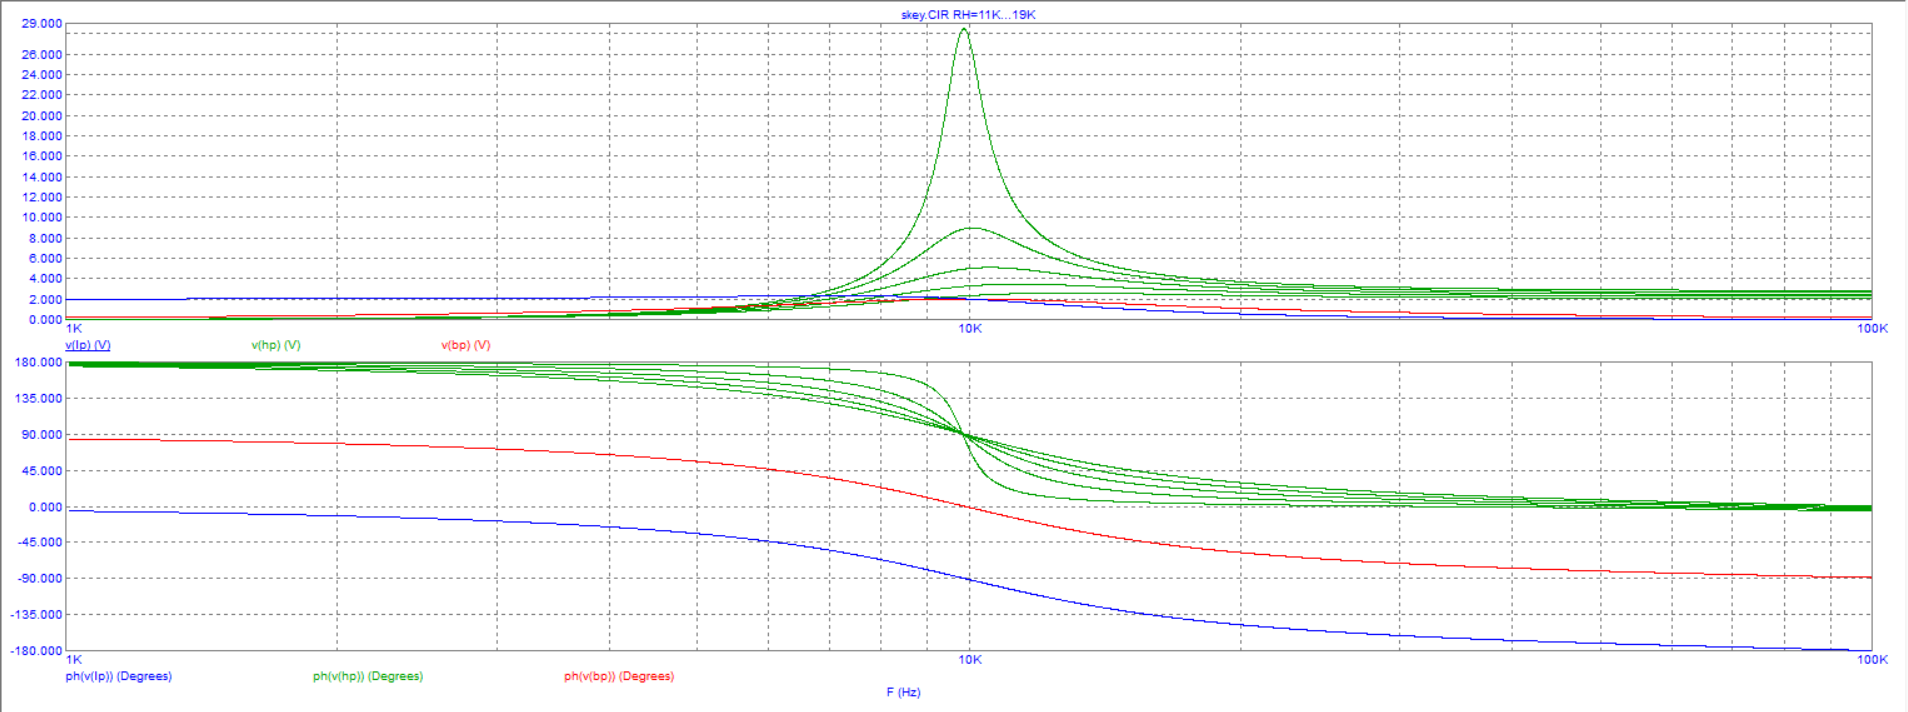
\includegraphics[width=12cm]{pics/point4_1_var2.png}
    \caption{Варьирование $R_H = [11K, 19K | 2K]$}
    \label{}
\end{figure}




\begin{figure}[h!]
    \centering
    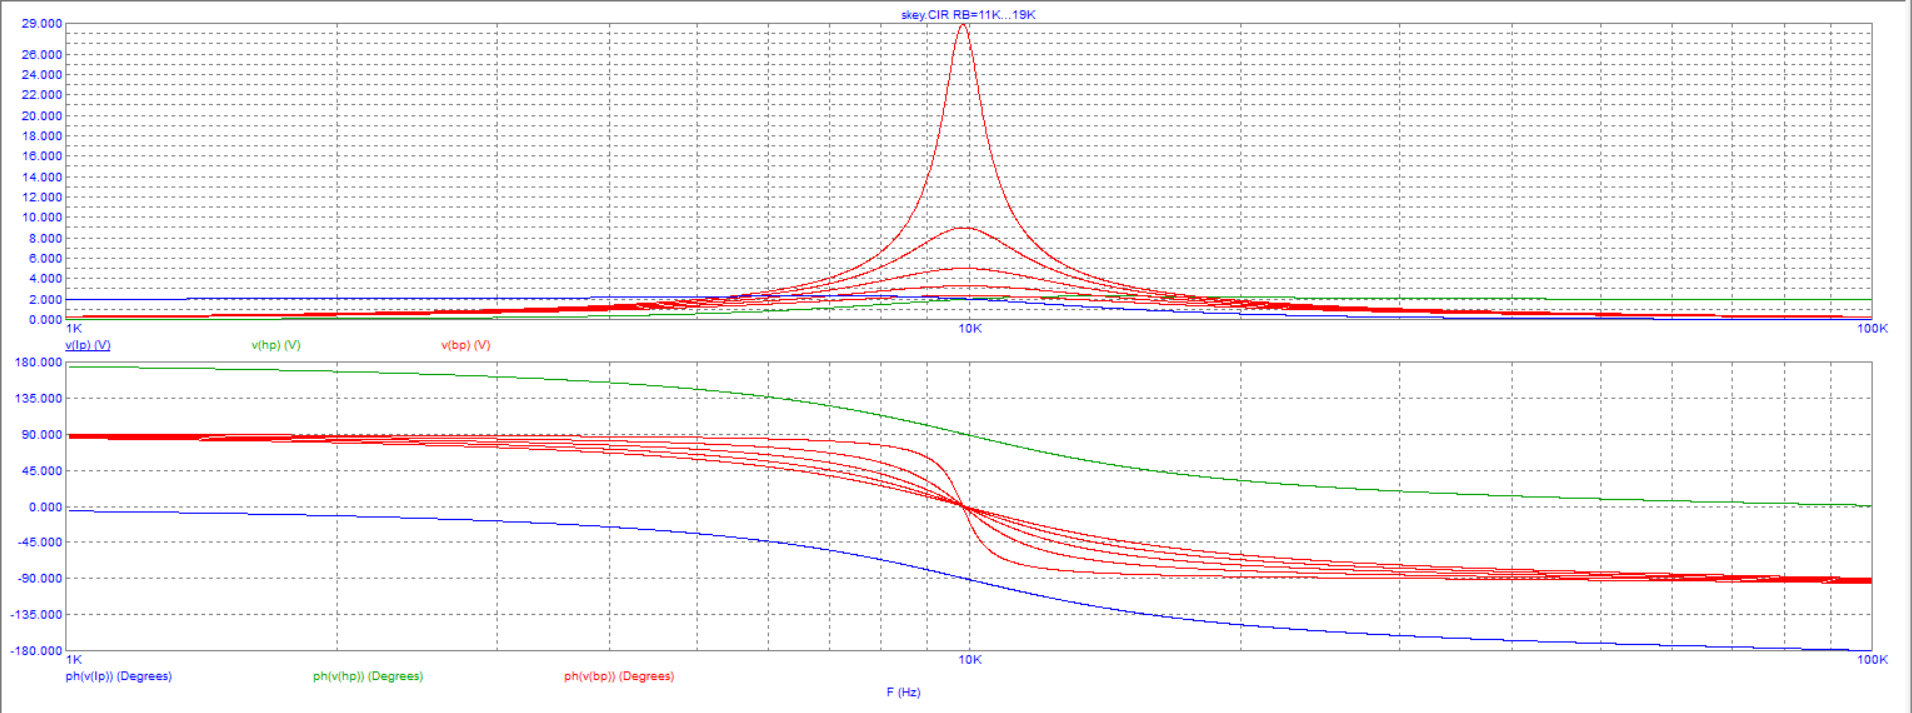
\includegraphics[width=12cm]{pics/point4_1_var3.png}
    \caption{Варьирование $R_B  = 11K, 19K | 2K]$}
    \label{}
\end{figure}




\begin{figure}[h!]
    \centering
    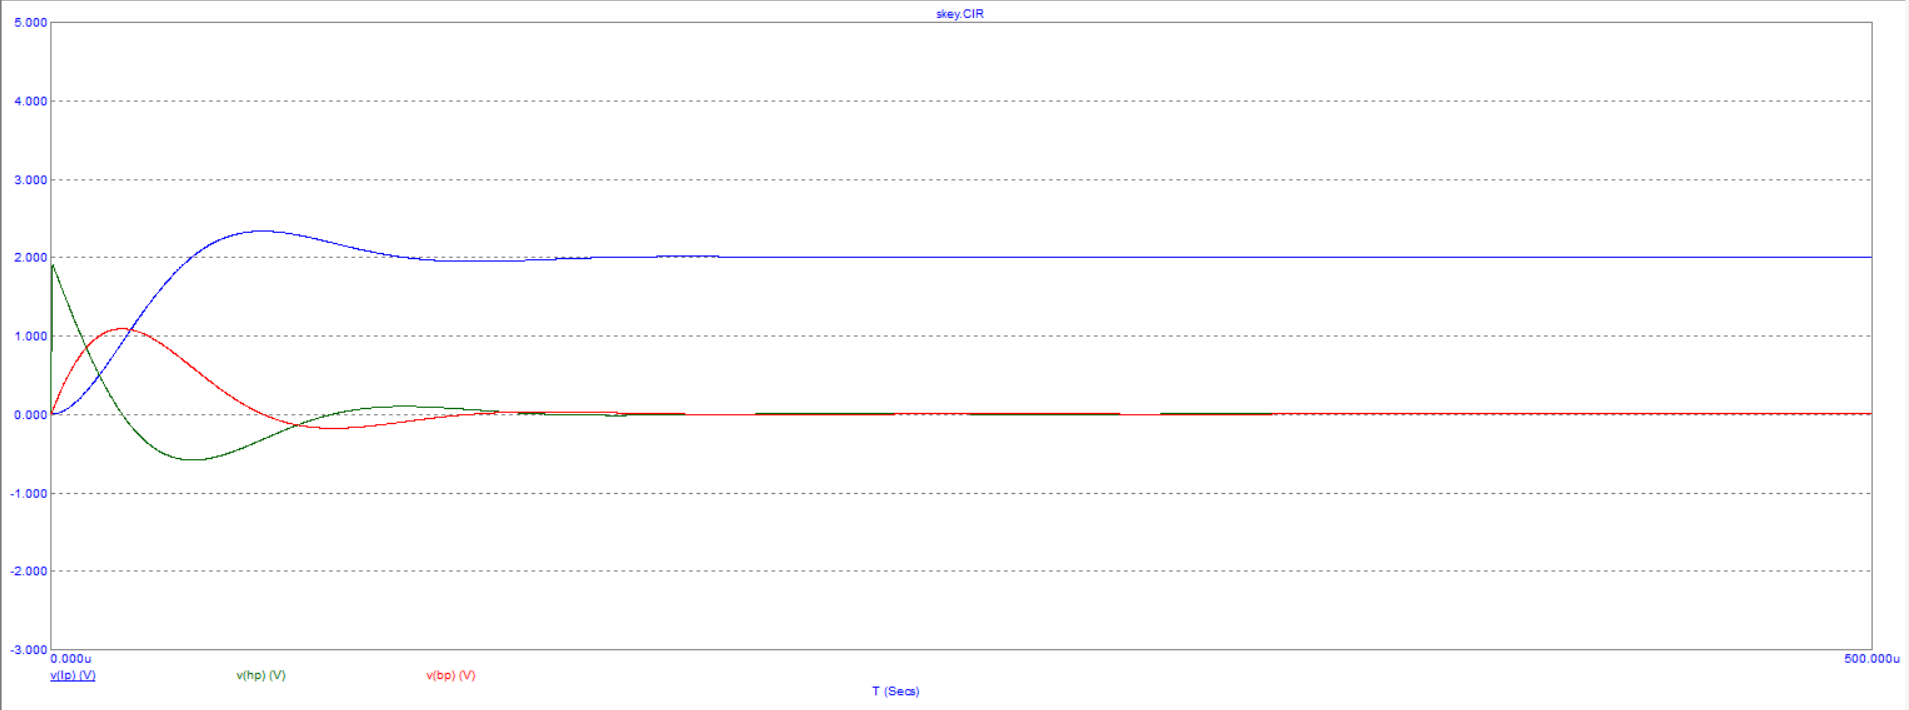
\includegraphics[width=12cm]{pics/point4_2.png}
    \caption{Варьирование $R_B  = 11K, 19K | 2K]$}
    \label{}
\end{figure}


\begin{figure}[h!]
    \centering
    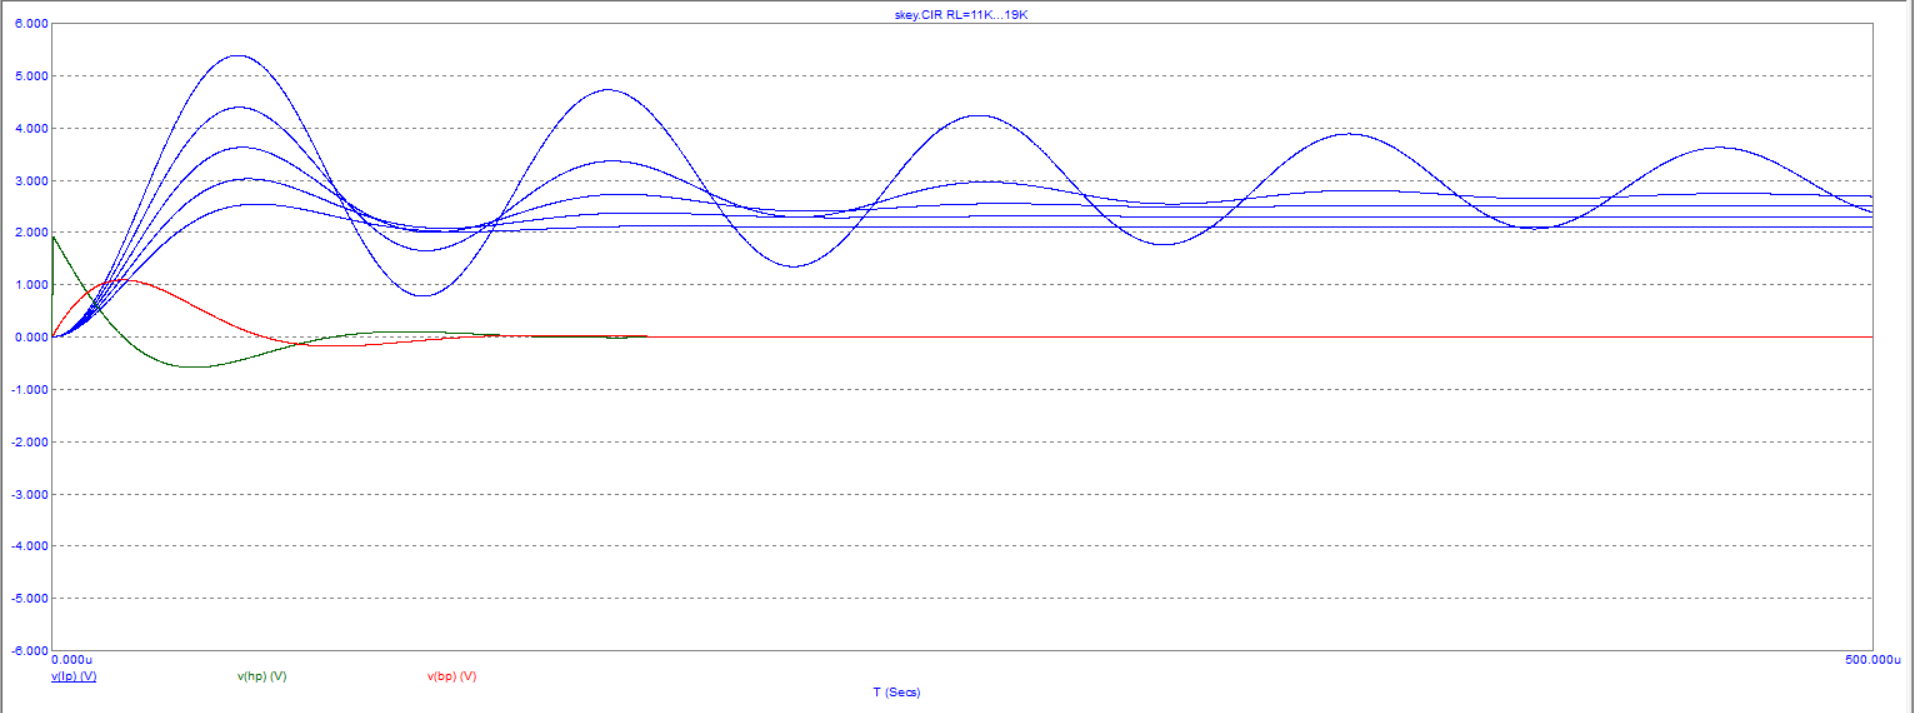
\includegraphics[width=12cm]{pics/point4_2_var1.png}
    \caption{Варьирование $R_B  = 11K, 19K | 2K]$}
    \label{}
\end{figure}



\begin{figure}[h!]
    \centering
    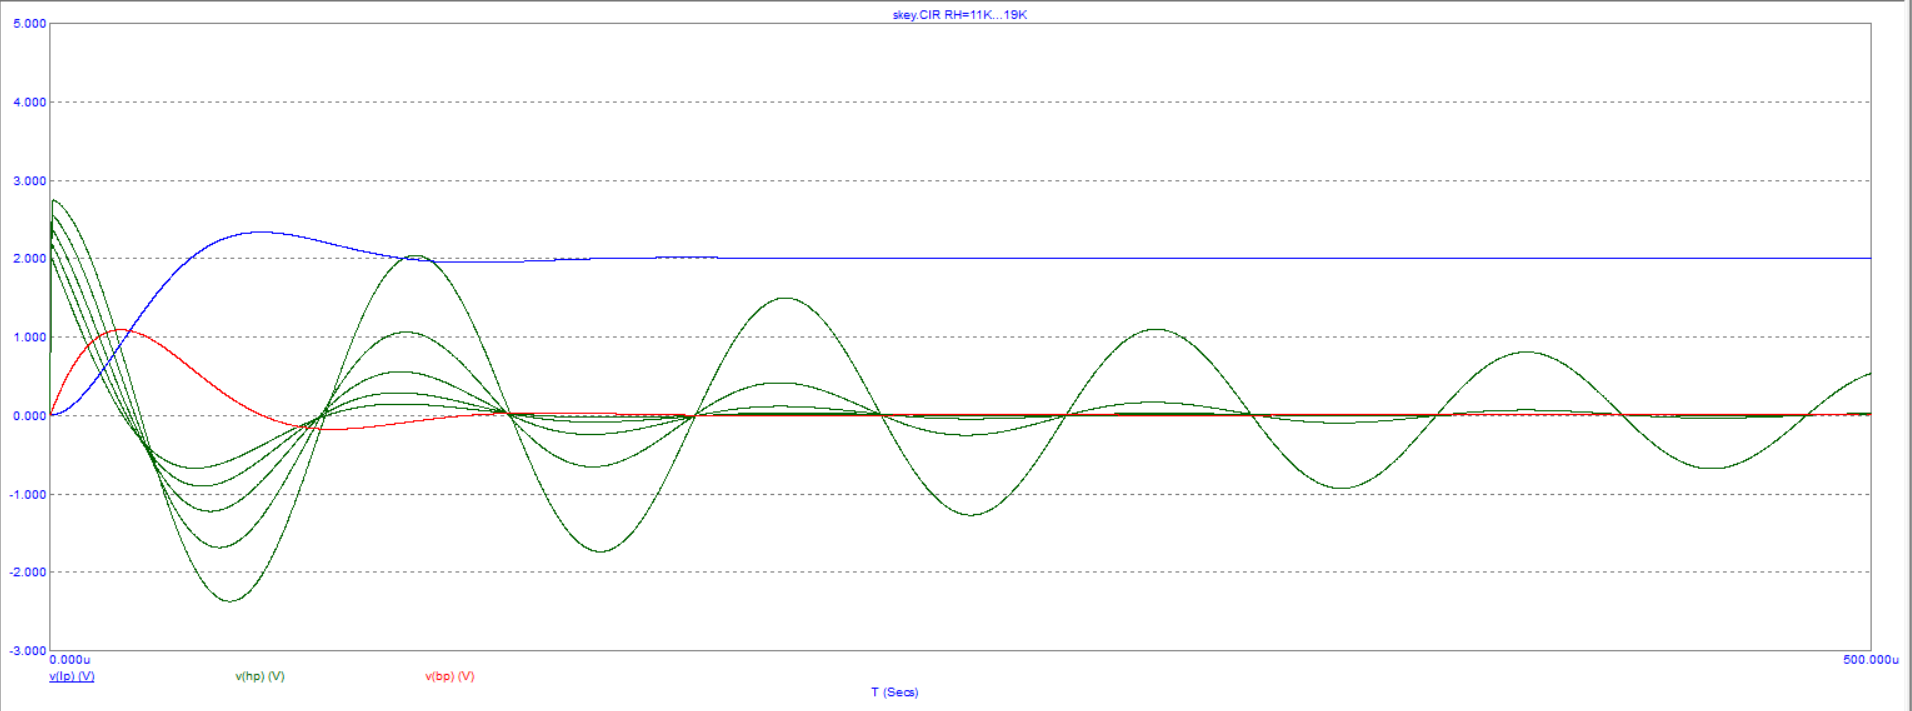
\includegraphics[width=12cm]{pics/point4_2_var2.png}
    \caption{Варьирование $R_B  = 11K, 19K | 2K]$}
    \label{}
\end{figure}


\begin{figure}[h!]
    \centering
    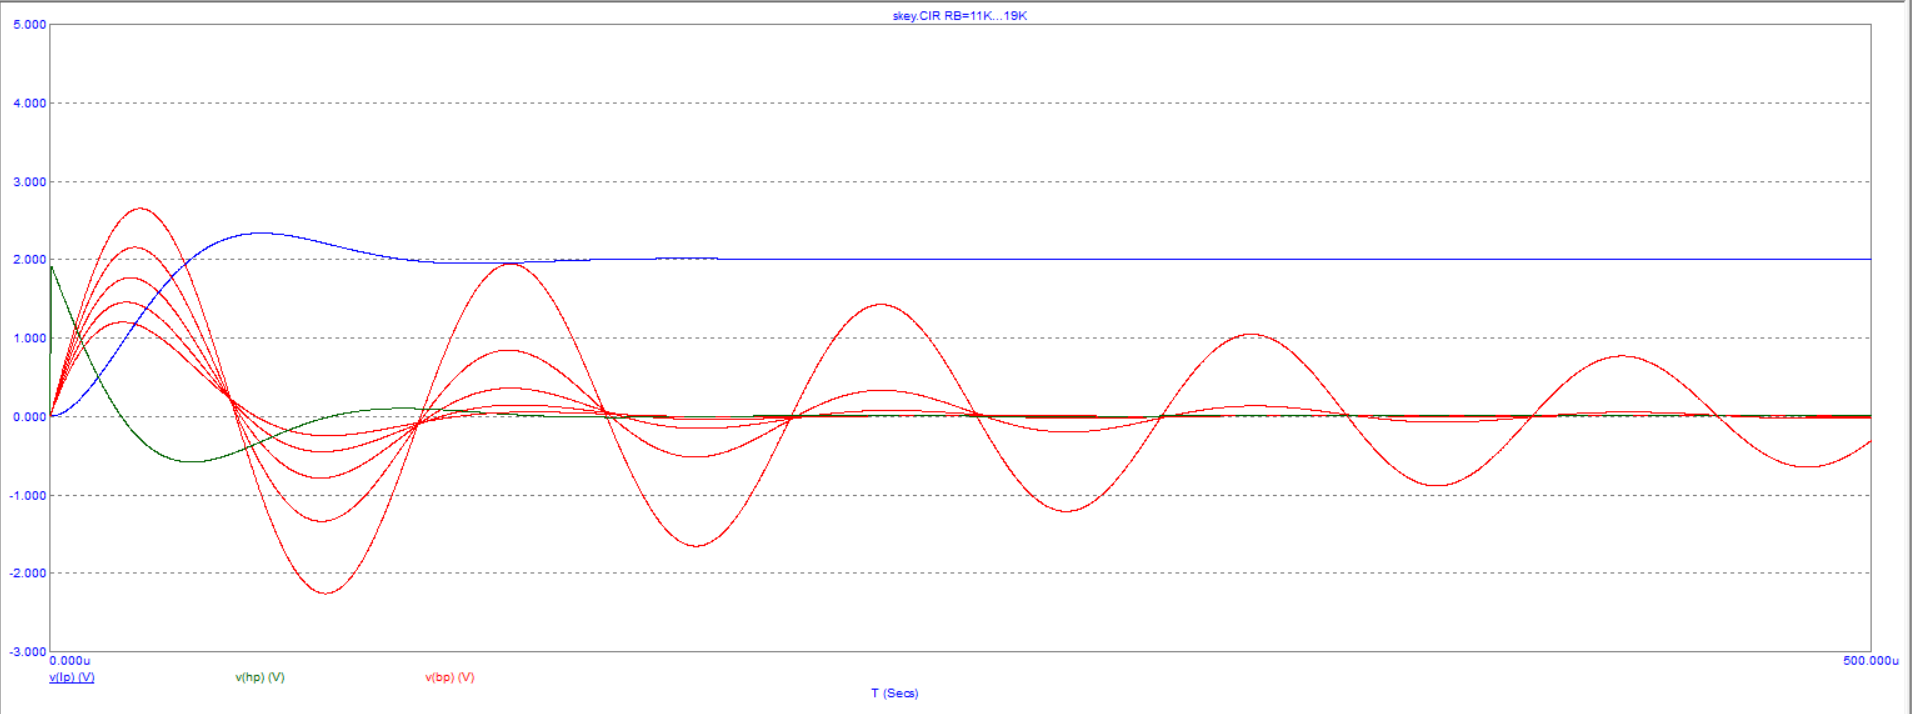
\includegraphics[width=12cm]{pics/point4_2_var3.png}
    \caption{Варьирование $R_B  = 11K, 19K | 2K]$}
    \label{}
\end{figure}


\begin{figure}[h!]
    \centering
    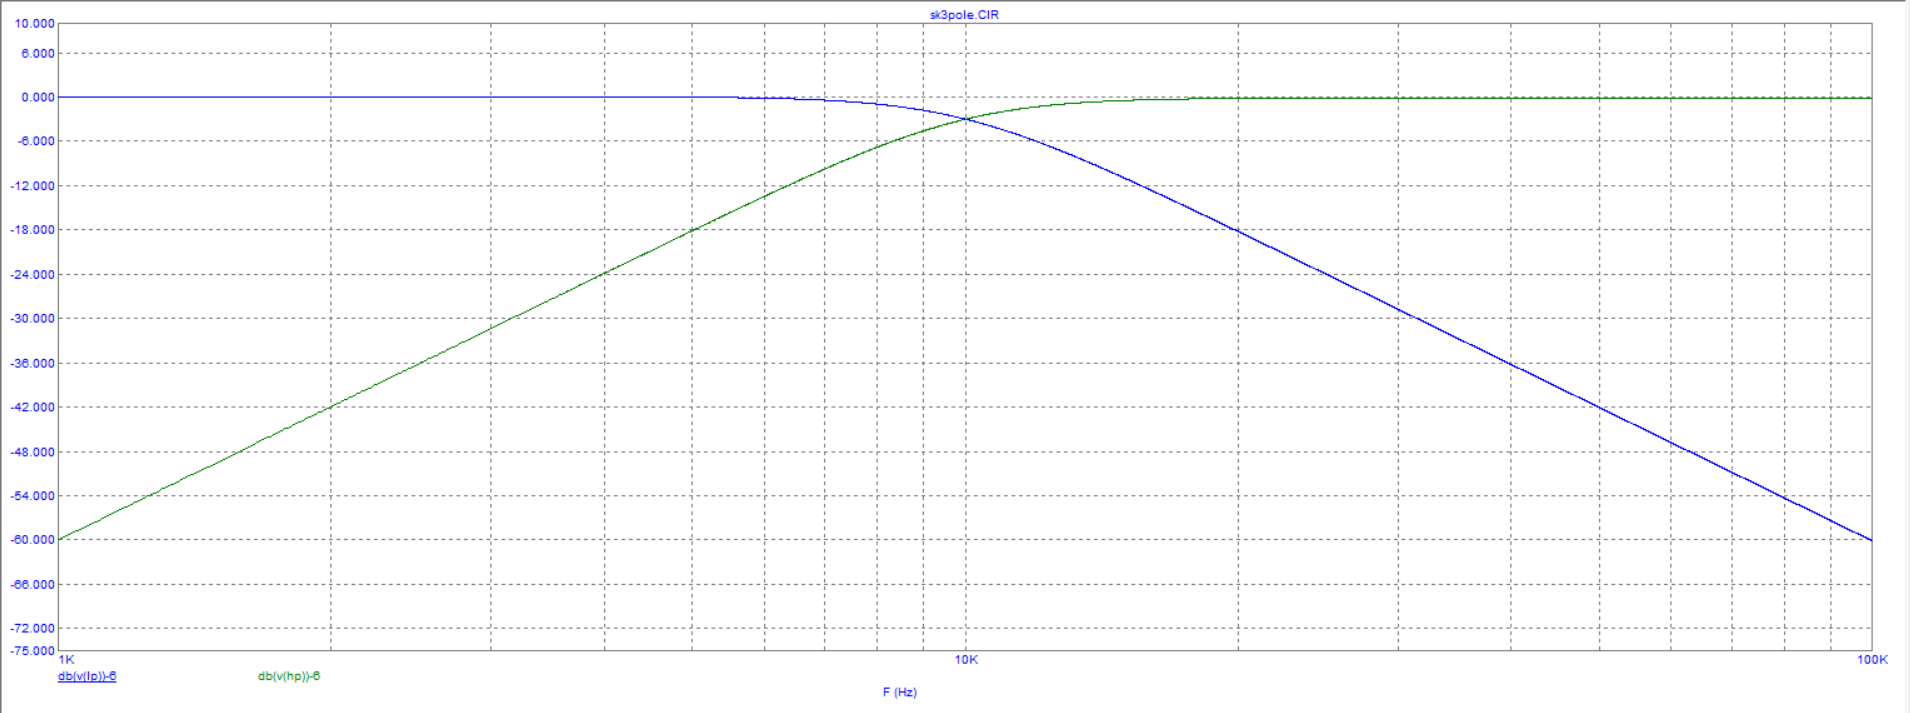
\includegraphics[width=12cm]{pics/point4_3.png}
    \caption{Варьирование $R_B  = 11K, 19K | 2K]$}
    \label{}
\end{figure}





\end{document}



 